\documentclass{article}
\usepackage[utf8]{inputenc}
\usepackage[russian]{babel}
\usepackage{marginnote}
\usepackage{graphicx}
\usepackage{float}

\title{Базы данных, лекция 10}
\author{@mikhirurg}
\date{April 2020}

\begin{document}

\maketitle

\section{Распределённая база данных}

"Узкое место" современных информационных систем и баз данных - это память. За все время развития информационных технологий в последние 20-30 лет мы не видели взрывного роста скорости доступа к данным со стороны носителей информации. Носители информации с быстрым доступом имеют высокую стоимость. В результате этого появилась идея распределения данных по нескольким носителям информации.
\newline \textit{Распередлённая БД} - это набор логически связанных между собой разделяемых данных и их описаний, которые физически распределены по нескольким вычислительным узлам некоторой сети.
\newline Такая база данных, в отличие от распределёной файловой системы, имеет высокоуровневый доступ к данным и модель данных.

\subsection{Фрагментация данных}
\begin{itemize}
    \item Горизонтальное фрагментирование
    \newline \textit{фрагментация по хронологическому порядку появления данных.}
    \item Вертикальное фрагментирование 
    \newline \textit{Пример: таблица пользователей, фрагментация по столбцам.
    \newline какая-то информация о пользователе требуется реже другой.}
    \item Репликация фрагментов 
    \newline Необходимо поддерживать актуальность копий
\end{itemize}

\subsection{Стратегии размещения данных}
\begin{itemize}
    \item Раздельное (фрагментированное) размещение.
    \newline \textit{Потеря связи с одним узлом, нарушает работу всей системы
    \newline Низкая скорость доступа}
    \item Размещение с полной репликацией
    \newline \textit{Копирование всей базы данных во всех узлах.}
    \item Размещение с выборочной репликацией
    \newline \textit{Необходима оптимальная стратегия размещения данных}
\end{itemize}

\subsection{Распределённая СУБД}

Распределённая СУБД - это rомплекс программ, предназначенный для управления распределённой БД и позволяющий сделать распределённость информации "прозрачной" для конечного пользователя.
\newline Виды прозрачности:
\begin{itemize}
    \item Прозрачность фрагментации
    \item Прозрачность расположения фрагмента
    \item Прозрачность количества реплик фрагмента
    \item Прозрачность контроля доступа
\end{itemize}
Гомогенные и гетерогенные распределённые СУБД: разделение по модели хранения данных в узлах.
\newpage
\subsection{12 правил распределённой БД от К. Дейта}
\begin{figure}[H]
    \centering
    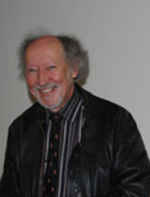
\includegraphics[width = .5\linewidth]{img0}
    \caption{Кристофер Дейт}
  \end{figure}
\begin{enumerate}
    \item Локальная автономность
    \item Отсутствие опоры на центральный узел
    \newline \textit{Не должно быть одного узла, который бы распределял данные между другими.}
    \item Непрерывное функционирование
    \newline \textit{Не должно быть плановых остановок системы.}
    \item Независимость от расположения
    \item Независимость от фрагментации
    \item Независимость от репликации
    \item Обработка расперделённых запросов
    \newline \textit{Работа с несколькими узлами}
    \item Обработка распределённых транзакций
    \item Независимость от типа оборудования
    \item Независимость от сетевой архитектуры
    \item Независимомть от операционной системы
    \item Независимость от типа СУБД
\end{enumerate}

\subsection{Распределённые запросы}
Обработка распределённого запроса:
\begin{itemize}
    \item Определение фрагмента
    \item Определение реплики фрагмента
    \item Определение местоположений постороения временных структур данных и маршрутеризация данных
\end{itemize}

Распределённые транзакци. Двухфазное завершения транзакций.
\newline Необходиимо получить подтверждение от узлов о благополучном завершении транзакции.

\subsection{Преимущества распределённых БД}

\begin{itemize}
    \item Отражение структуры организации
    \item Разделяемость и локальная автономность
    \item Повышение доступности данных
    \item Повышение надёжности
    \item Повышение производительности
    \item Модульность системы
\end{itemize}

\subsection{Недостатки распределённых БД}

\begin{itemize}
    \item Повышение сложности
    \item Увеличение стоимости
    \item Сложности в обеспечении защиты
    \item Сложности в обеспечении целостности данных
    \item Высокая стоимость стандартизации и поддержки стандартов
\end{itemize}

\end{document}
